\subsection{Proceso Interno 15: Mostrar Resultados}

\subsubsection{Objetivo de la Actividad}
El propósito principal de la actividad \textbf{``Mostrar Resultados''} es presentar de manera clara y comprensible al usuario final, a través de la interfaz gráfica (UI), la solución óptima encontrada por el Algoritmo Bioinspirado al concluir el proceso de optimización. Esto incluye el mejor conjunto de parámetros (ej.\ masas finales optimizadas) y su correspondiente valor de fitness, definido como el Exponente de Lyapunov ($LE$) minimizado. Opcionalmente, puede incluir una visualización final estática de la trayectoria asociada a la solución óptima.

\subsubsection{Entradas Principales}
\begin{itemize}
    \item \textbf{Señal de finalización}: Evento que indica término del proceso de optimización
    \item \textbf{Parámetros óptimos}: Valores numéricos finales (ej.\ masas de cuerpos)
    \item \textbf{Valor de fitness}: $LE$ asociado a la solución óptima
    \item \textbf{Datos de trayectoria (opcional)}: Posiciones/velocidades de la simulación REBOUND
    \item \textbf{Resumen de optimización (opcional)}: Detalles del proceso de optimización
\end{itemize}

\subsubsection{Sub-pasos Secuenciales}
Este apartado es proporcionado para profundizar y describir de forma textual cada paso contenido dentro del diagrama del proceso descrito en la figura~\ref{fig:process_diagram15}.
\subsubsection*{1. Recibir Señal de Finalización}
\begin{itemize}
    \item UI detecta notificación de término del Algoritmo Bioinspirado
\end{itemize}

\subsubsection*{2. Recibir Datos Finales}
\begin{itemize}
    \item Datos recibidos incluyen:
    \begin{itemize}
        \item Parámetros óptimos (valores numéricos)
        \item $LE$ final
        \item Bandera de existencia de datos de trayectoria
        \item Resumen de optimización (si está disponible)
    \end{itemize}
\end{itemize}

\subsubsection*{3. Formatear Datos para Presentación}
\begin{itemize}
    \item Conversión a formatos legibles:
    \begin{itemize}
        \item Parámetros: $\text{valor} \to \text{cadena}$ (ej.\ \texttt{``0.1234''})
        \item $LE \to \texttt{``LE: -0.567''}$
        \item Generación de etiquetas descriptivas (ej.\ \texttt{``Masa Cuerpo 1 Final:\~''})
        \item Resumen $\to$ texto descriptivo (ej.\ \texttt{``50 generaciones''})
    \end{itemize}
\end{itemize}

\subsubsection*{4. Manejar Visualización Final (Condicional)}
\begin{enumerate}[label=Condición \arabic*:]
    \item Verificar existencia de datos de trayectoria
    \item Confirmar configuración de visualización habilitada
\end{enumerate}

\textbf{Si ambas condiciones se cumplen:}
\begin{itemize}
    \item Preparación de datos:
    \begin{itemize}
        \item Extracción de posiciones/velocidades
        \item Determinación de escalas (ej.\ rango de coordenadas)
        \item Generación de metadatos (etiquetas ejes, título)
    \end{itemize}
    \item Llamado al \texttt{Módulo de Visualización}
    \item Integración del gráfico en UI
\end{itemize}

\textbf{Si falla alguna condición:}
\begin{itemize}
    \item Mostrar solo resultados textuales
\end{itemize}

\subsubsection*{5. Presentar Resultados en Pantalla}
\begin{itemize}
    \item Actualización de elementos UI:\
    \begin{itemize}
        \item Parámetros óptimos formateados con etiquetas
        \item $LE$ con interpretación (ej.\ \texttt{``indica estabilidad''})
        \item Resumen de optimización (si existe)
        \item Gráfico estático (si se generó)
    \end{itemize}
    \item Habilitación de controles:
    \begin{itemize}
        \item Botones \texttt{Guardar}, \texttt{Reiniciar}, \texttt{Cerrar}
    \end{itemize}
\end{itemize}

\subsubsection*{6. Esperar Interacción del Usuario}
\begin{itemize}
    \item UI permanece en estado receptivo para acciones posteriores
\end{itemize}

\subsubsection{Lógica Interna y Decisiones}
\begin{itemize}
    \item \textbf{Decisión clave}: Generar visualización gráfica
    \begin{itemize}
        \item Depende de:
        \begin{enumerate}[label=~(\alph*)]
            \item Datos de trayectoria disponibles
            \item Configuración de visualización activada
        \end{enumerate}
    \end{itemize}
    \item \textbf{Manejo de opcionales}:
    \begin{itemize}
        \item Omisión automática de secciones sin datos
    \end{itemize}
\end{itemize}

\subsubsection{Manejo de Datos Específico}
\begin{itemize}
    \item \textbf{Entradas}:
    \begin{itemize}
        \item Parámetros: \texttt{float/double}
        \item $LE$: \texttt{float/double}
        \item Trayectoria: \texttt{arrays/listas} (opcional)
    \end{itemize}
    \item \textbf{Intermedios}:
    \begin{itemize}
        \item Cadenas formateadas
        \item Datos gráficos procesados
    \end{itemize}
    \item \textbf{Salidas}:
    \begin{itemize}
        \item Texto UI formateado
        \item Gráfico estático (opcional)
    \end{itemize}
\end{itemize}

\subsubsection{Salidas Principales}
\begin{itemize}
    \item UI actualizada con:
    \begin{itemize}
        \item Resultados numéricos y textuales
        \item Visualización gráfica (condicional)
        \item Controles interactivos habilitados
    \end{itemize}
\end{itemize}

\subsubsection{Interacciones Internas}
\begin{itemize}
    \item \textbf{Con Algoritmo Bioinspirado}:
    \begin{itemize}
        \item Recepción asincrónica de datos finales
    \end{itemize}
    \item \textbf{Con UI}:
    \begin{itemize}
        \item Actualización dinámica de componentes visuales
    \end{itemize}
    \item \textbf{Con Módulo de Visualización}:
    \begin{itemize}
        \item Integración gráfica bajo demanda
    \end{itemize}
\end{itemize}
\newpage
\subsubsection{Diagrama del Proceso}
\begin{figure}[H]
    \centering
    \adjustbox{max width=\textwidth, max height=0.9\textheight}{%
        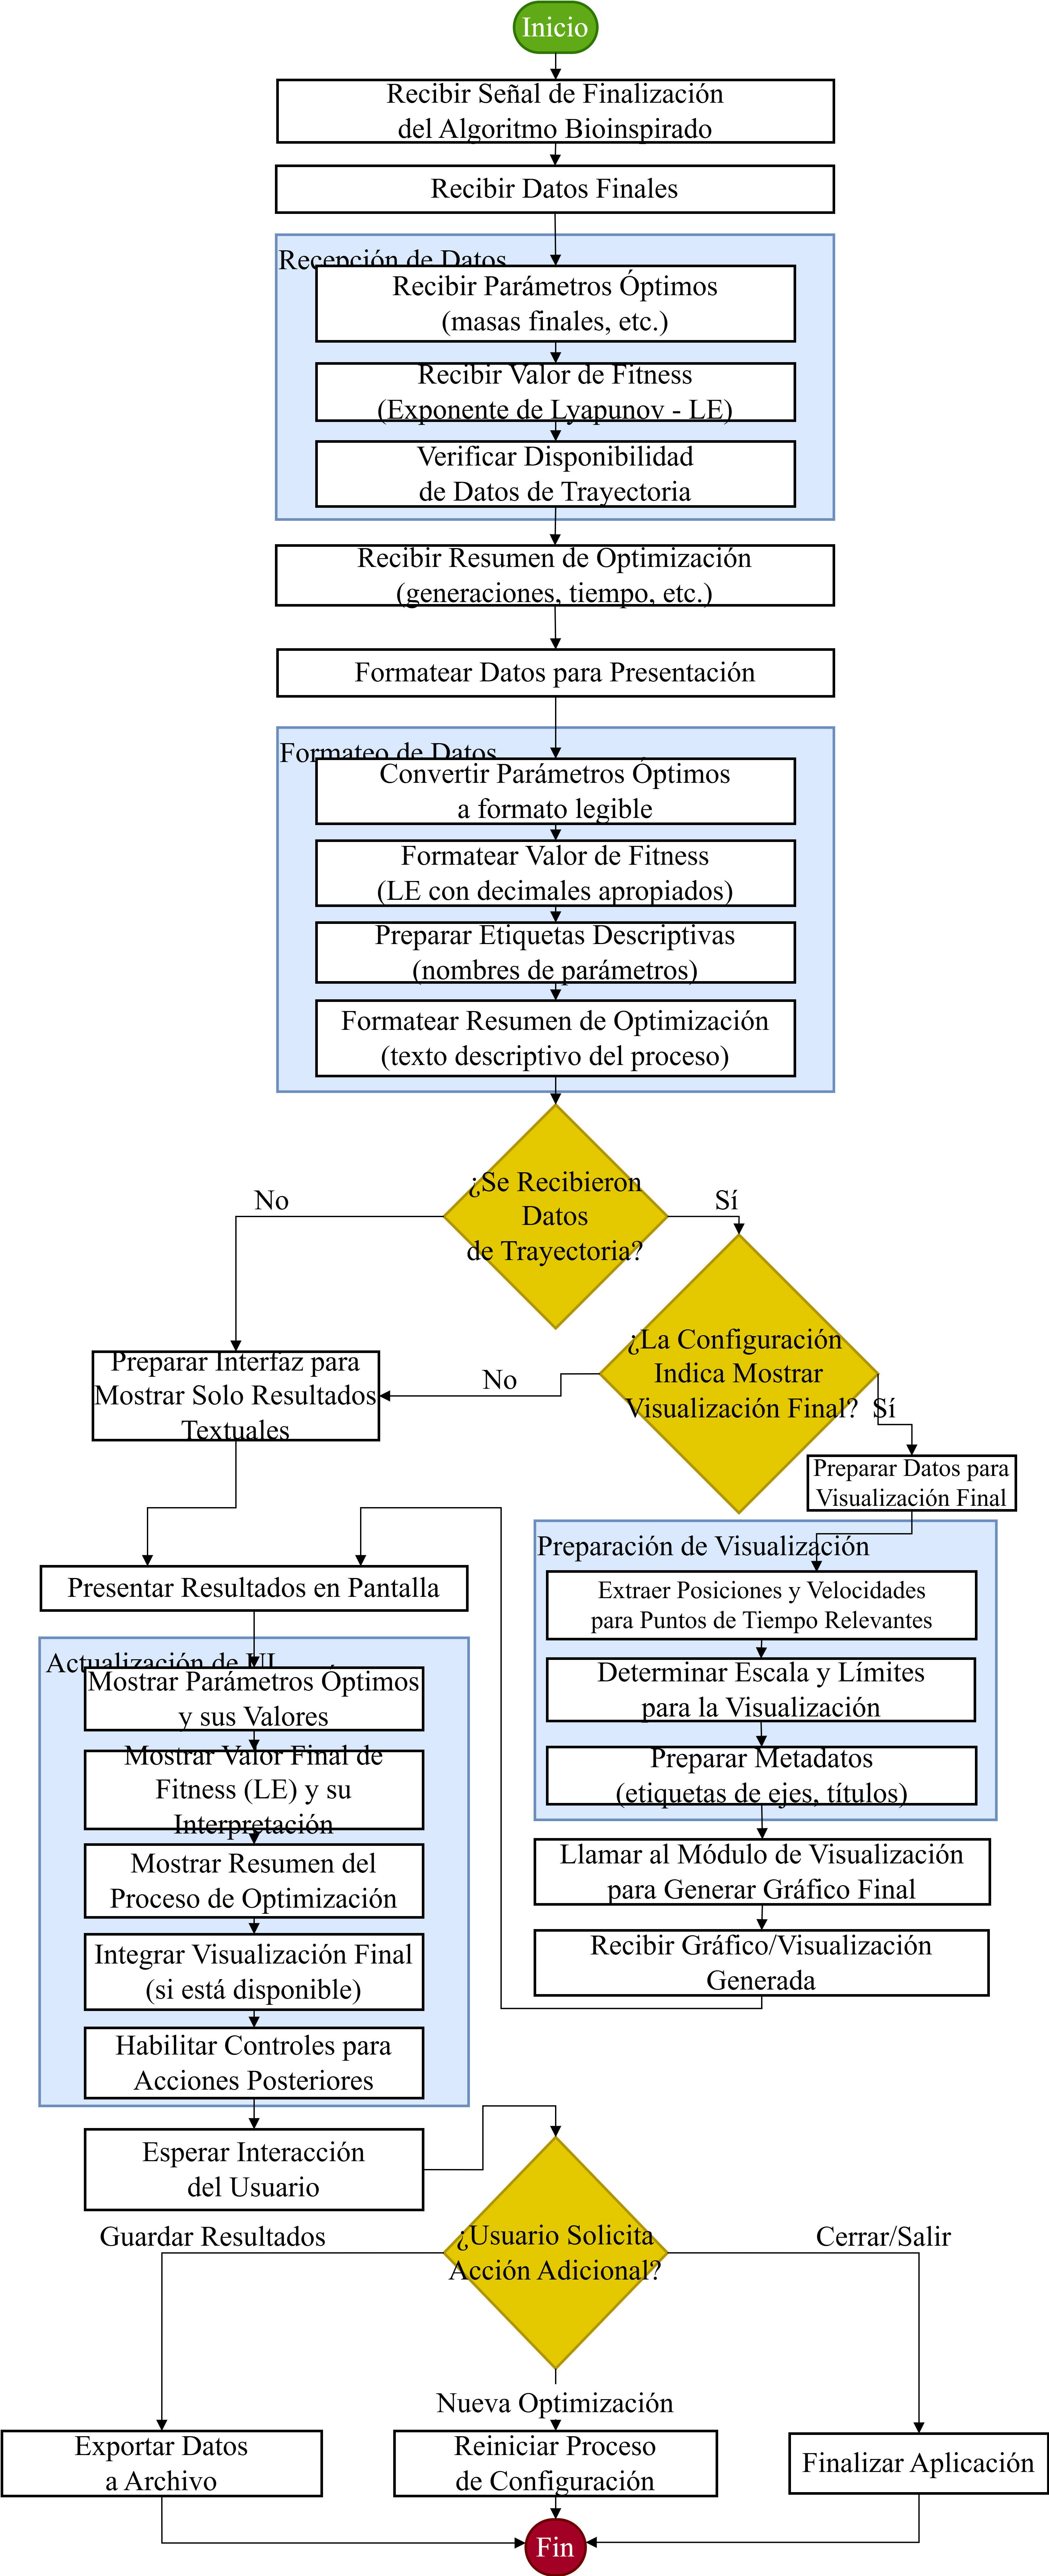
\includegraphics{img/Analisis/DiagramaProcesos/DiagramaProceso15_Proceso Interno_Mostrar Resultados.png}
    }
        \caption{Diagrama de Proceso Interno 15: Mostrar Resultados}%
    \label{fig:process_diagram15}
\end{figure}
\newpage